\chapter{Walidacja rozwiązania}
\label{cha:tests}
Po wstępnym nastrojeniu układu, należy uruchomić oraz przetestować urządzenie. Autor zapoznał się w~tym celu z~normą dotyczącą mierzenia poziomu natężenia hałasu \cite{test_norm}, jednak ze względów subiektywnych zastosował się jedynie do zaleceń traktujących o~metodzie pomiarowej, nie zaś do dokładnego sposobu wykonania pomiaru. Zarówno sposób, jak i~wyniki pomiarów, opisane są w~sekcji \ref{sec:practical_test}.
\section{Układ symulowany w środowisku MATLAB/Simulink}
Celem zbadania zachowania algorytmu, autor utworzył model filtra FIR-LMS w~środowisku obliczeniowym MATLAB/Simulink. Model ukazano na rysunku \ref{fig:model_rys}.
\begin{figure}[h!]
	\centering
	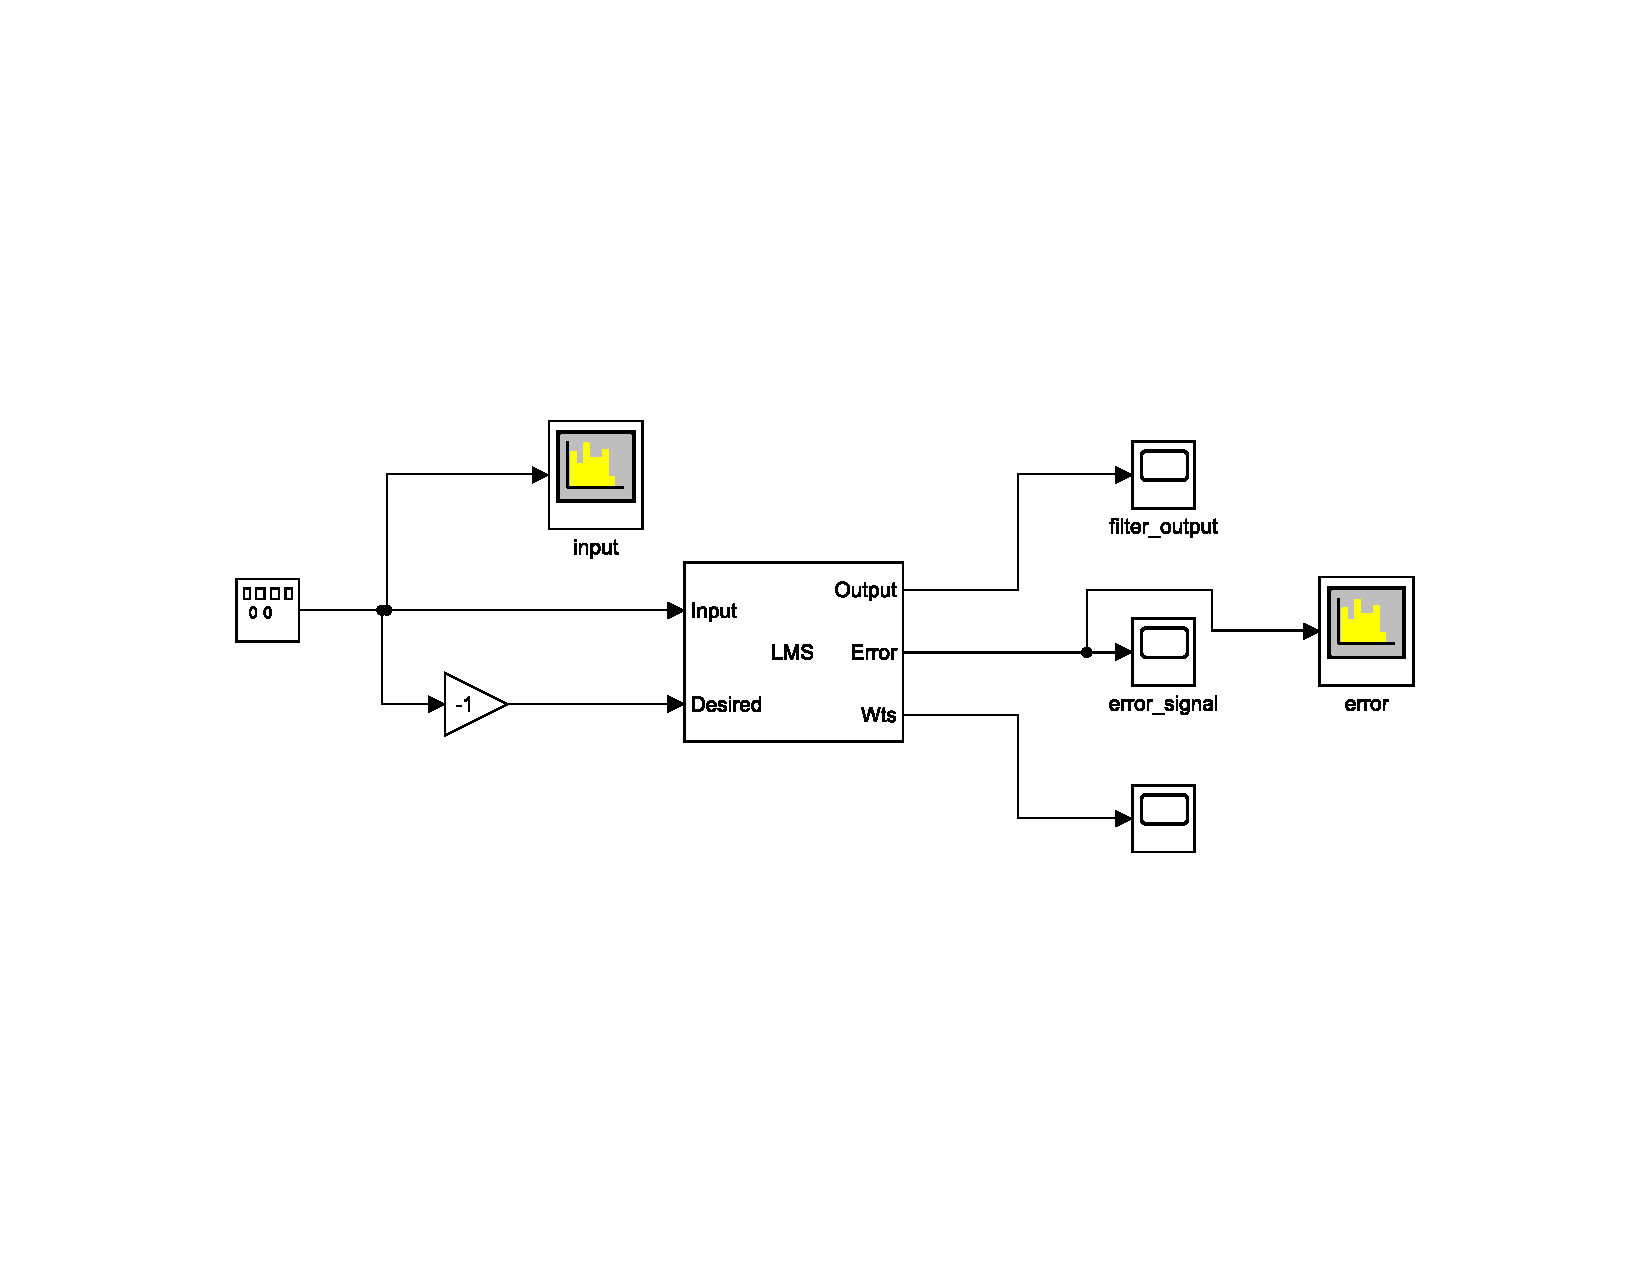
\includegraphics[scale=0.5]{../Assets/model_anc_rys.pdf}
	\caption{Schemat modelu algorytmu aktywnego tłumienia hałasu wykonanego w~pakiecie MATLAB/Simulink.}
	\label{fig:model_rys}
\end{figure}

Jako wejście główne podano losowo generowany sygnał, zaś jako wejście sygnału pożądanego podano odwrotność głównego sygnału. Następnie, autor wyświetlił na blokach ,,Scope'' wartości sygnałów wyjściowych. PLACEHOLDER odnośnie dodatkowych rzeczy czyli wykresy itp.

\section{Test praktyczny}
\label{sec:practical_test}
Celem sprawdzenia jakości zbudowanego urządzenia, autor dokonał testu praktycznego, w~którym zmierzył poziom natężenia dźwięku w~pewnym pomieszczeniu ze stałym, powtarzalnym typem hałasu, w~trzech wariantach -- bez tłumienia, tylko z~tłumieniem pasywnym, oraz z~tłumieniem pasywnym i~uruchomionym tłumieniem aktywnym pochodzącym z~zaprogramowanego układu.
\subsection{Warunki testu}
\label{subsec:circumstances}
Układ został przetestowany w~pomieszczeniu monitoringowym przeznaczonym dla ochrony biurowca. Pomieszczenie jest niewielkie i~znajduje się w~nim wiele urządzeń elektrycznych -- komputery, monitory, wiatraki, zasilacze oraz szafka z~urządzeniami sieciowymi, których układy chłodzące generują dość uciążliwy przy długotrwałej ekspozycji hałas. Pokój, który wykorzystano do testów, znajduje się na uboczu budynku, z~dala od pomieszczeń biurowych, gdzie znajdują się pracownicy. Pozwala to zatem na przetestowanie działania układu przy powtarzalnym hałasie o~niskiej częstotliwości. Pewne dźwięki oczywiście mimo wszystko przedostaną się do pokoju, nie będą jednak głównym elementem składowym danego typu hałasu mierzonego w~tym pomieszczeniu. Urządzenie umieszczono w~środku pomieszczenia i~skierowano je mikrofonem w~stronę szafki z~urządzeniami sieciowymi, które w~tym teście są głównym źródłem hałasu. Odległość od źródła dźwięku wynosiła PLACEHOLDER, %TODO ILE METRÓW???? 
zaś czas pomiaru wynosił minutę dla każdego z~etapów.
\subsection{Typowe rodzaje hałasu}
Jak już wspomniano w~sekcji \ref{sec:hałas} rozdziału \ref{cha:teoria}, typowymi rodzajami hałasu, które można chcieć tłumić takim urządzeniem, są:
\begin{itemize}
	\item rozmowy pobliskich osób,
	\item szum wentylacyjny,
	\item dźwięk towarzyszący pracy silnika.
\end{itemize}
Są to zatem sygnały charakteryzujące się (w~przybliżeniu) stałym przedziałem częstotliwościowym i~niewielkim natężeniem, jednak będące uciążliwymi w~dłuższej perspektywie czasowej. W~ramach testu praktycznego sprawdzono działanie układu przy ekspozycji na hałas pochodzący od rozmowy kilku osób w~biurze oraz na szum wentylatorów i~pobliskich urządzeń elektrycznych.
\subsection{Poziom hałasu bez tłumienia}
Pomiaru bez tłumienia dokonano przy otwartej muszli słuchawek i~wyłączonym algorytmie. Zbierano dane z~mikrofonu odsłuchowego (feedback). Pozwoliło to na zebranie danych o~poziomie natężenia hałasu w~miejscu, w~którym znajdowało się urządzenie. Przy założeniu opisanych w~sekcji \ref{subsec:circumstances} warunków testu, średni poziom hałasu zmierzony bez żadnego sposobu tłumienia wyniósł PLACEHOLDER. %TODO uzupełnić pomiar.
Widmo częstotliwościowe pokazano na rysunku \ref{fig:widmo_bez}.
\begin{figure}[h!]
	\centering
	\includegraphics{../Assets/widmo_bez_tlumienia.png}
	\caption{Widmo częstotliwościowe hałasu przy pomiarze bez tłumienia hałasu.}
	\label{fig:widmo_bez}
\end{figure}

\subsection{Poziom hałasu z pasywnym tłumieniem}
Następnie, aby dokonać pomiaru natężenia hałasu przy pasywnym tłumieniu, zamknięto i~zebrano dane pochodzące z~drugiego mikrofonu (feedback). Dzięki temu otrzymano informację o~tym, jaki poziom hałasu panuje wewnątrz słuchawki, czyli jaki hałas słyszałby użytkownik przy użyciu jedynie pasywnego tłumienia, które dają użyte nauszniki. Przy tych samych założeniach, średni poziom hałasu wyniósł PLACEHOLDER2. %TODO uzupełnić pomiar.
Widmo częstotliwościowe zaprezentowano na rysunku \ref{fig:widmo_pasywnie}. 
\begin{figure}[h!]
	\centering
	\includegraphics{../Assets/widmo_pasywnie.png}	
	\caption{Widmo częstotliwościowe hałasu przy pomiarze z~pasywnym tłumieniem.}
	\label{fig:widmo_pasywnie}
\end{figure}

\subsection{Poziom hałasu z aktywnym tłumieniem}
Ostatecznie, aby dowieść skuteczności rozwiązania, uruchomiono algorytm i~ponownie zebrano dane z~mikrofonu odsłuchowego. Średni poziom hałasu zmierzony w~ten sposób wyniósł PLACEHOLDER3. %TODO uzupełnić pomiar.
Widmo częstotliwościowe zamieszczono na rysunku \ref{fig:widmo_aktywnie}.
\begin{figure}[h!]
	\centering
	\includegraphics{../Assets/widmo_aktywnie.png}	
	\caption{Widmo częstotliwościowe hałasu przy pomiarze z~aktywnym tłumieniem.}
	\label{fig:widmo_aktywnie}
\end{figure}

Dodatkowo, aby porównać zbudowany układ do istniejącego rozwiązania rynkowego, ten sam pomiar wykonano dla słuchawek Jabra Elite~80. Tak jak urządzenie autora, używają one podejścia feedforward-feedback.\cite{JabraEvolve80} Sposób realizacji rozwiązania (analogowy czy cyfrowy) nie jest nigdzie wyjawiony, można jednak domniemywać użycie analogowego toru tłumienia ze względu na dużo niższe zużycie energii elektrycznej oraz wymiary takiego układu. Słuchawki podłączono do komputera osobistego i~umieszczono w~tym samym miejscu, w~którym wcześniej mierzono urządzenie autora. Sygnał z~wnętrza słuchawek zbierano poprzez włożenie do muszli słuchawek komercyjnych mikrofonu odsłuchowego z~urządzenia autora (wciąż podpiętego do mikrokontrolera) i~przesyłanie danych z~niego (za pośrednictwem modułu komunikacji UART) do komputera monitorującego test. Średni poziom hałasu wewnątrz słuchawek firmowych zmierzony w~ten sposób wyniósł PLACEHOLDER4. Widmo częstotliwościowe tak zmierzonego dźwięku pokazano na rysunku \ref{fig:widmo_jabra}.
\begin{figure}[h!]
	\centering
	\includegraphics{../Assets/widmo_jabra.png}	
	\caption{Widmo częstotliwościowe hałasu przy pomiarze z~aktywnym tłumieniem słuchawek komercyjnych Jabra Elite~80.}
	\label{fig:widmo_jabra}
\end{figure}
%TODO mikrofon z peceta do przestrzeni, zmierzyc widmo dzwieku do matlaba